%# -*- coding: utf-8-unix -*-
%%==================================================
%% chapter02.tex for SJTU Bachelor Thesis
%%==================================================

\chapter{技术背景}
\label{chap:RL}
\section{进程内存管理简述}
内存作为程序使用最频繁的计算机部件之一,为程序的内存和代码提供了存放空间,又为程序访问磁盘提供了缓存,提高了磁盘I/O的效率。可以说,对于任何一个程序,如果它不高效地使用内存,那么它的运行效率也将会十分低下。而Linux内核\cite{linux}对物理内存的利用更是精益求精。在开始本文的论述前,有必要对Linux程序如何使用内存有大致的了解。
\subsection{虚拟内存及其分布}
现代操作系统将物理内存抽象为一个私有的虚拟地址空间,使得物理内存可以被多个进程公平地使用,且不会相互写入对方的内存。Linux为每个进程提供了一个页表(Page Table),当进程被调度运行时,操作系统将CR3寄存器更新为进程页表的基地址。每一个CPU核都有一个MMU(内存管理单元),当CPU发出访存指令时,MMU接收CPU发来的虚拟地址,通过查询页表得知CPU发送的虚拟地址所对应的物理地址。虚拟地址空间的大小由系统的字宽来决定:对于一个32位的系统,CPU的访存能力是0 ~ $2^{32}-1$,故该系统下每个进程的虚拟地址空间大小为4G;而对于一个64位的系统,CPU的访存能力是0 ~ $2^{64}-1$,然而由于这是一个很大的数字,目前还没有程序可以使用到如此大的虚拟地址空间,故CPU访存仅使用48位,所以虚拟地址空间是$2^{48}$,即256T的虚拟地址空间。物理内存和其他存储层次中的存储设备一样,将自己划分为相同大小的块进行管理,一般为4KB,即4096个byte。相类似的,虚拟地址空间的管理单位也是4096KB。虚拟内存中每一个4K大小的块称为虚拟页,而物理内存中每一个4K大小的块称为物理页,或称为页帧。物理内存以页帧为单位和磁盘做数据交换,作为磁盘访问的缓存。每当CPU访问一个虚拟地址时,MMU将虚拟地址翻译为物理地址,再去内存的缓存中获取数据。如果获取不到,则会去内存中查找数据。相类似的,如果内存中也找不到该内存地址的数据,则会发生缺页异常(page fault),此时内核会调用page fault处理函数,从磁盘上读取相应数据,加载到内存中来。
\label{chap:mem}
Linux将每个进程的虚拟地址空间划分为许多部分,映射到不同的物理内存(或不映射到物理内存),具有不同的访问权限,存放着不同的数据,发挥着不同的功能。一个典型的用户态进程的虚拟地址空间按照从低地址到高地址的顺序,主要有以下几个部分,各部分之间不一定完全紧临:
\begin{itemize}
  \item 0 ~ 1G:保留段。
  \item 1G ~ ? :由execve()函数映射到虚拟地址空间的二进制文件。包含代码段(只有读权限),已初始化数据段(具有读写权限),未初始化数据段(有读写权限)。
  \item 运行时堆(heap),有读写权限,栈顶由brk指针指向,向上增长,同一进程中的线程共享,malloc()函数为线程分配这一区域的内存。
  \item 共享库的内存映射区,具有读权限,所有进程的虚拟地址空间映射着同一份共享库的代码和数据。
  \item 其他共享内存区,例如进程通过调用shmget获得的和其他进程共享的内存块。
  \item 用户栈区。具有读写权限。同一进程中的线程不共享。栈顶由当前线程的\%rsp寄存器指向,向下增长。由编译器决定是否将变量分配在栈中。
  \item 3G ~ ? :每个进程都相同的内核虚拟内存区域。包含所有进程共享的代码和数据,以及一块由所有进程共享的物理页面。其中最典型的例子是$struct file$,即文件描述符表。对于所有的文件,所有的进程共享其对应的$struct file$,这也意味着所有进程共享着文件读写位置。
  \item ?~ 4G:每个进程都不同的内核虚拟内存区域。包含所有进程独享的内核数据结构、内核栈。
\end{itemize}
\begin{figure}[!htp]
  \centering
  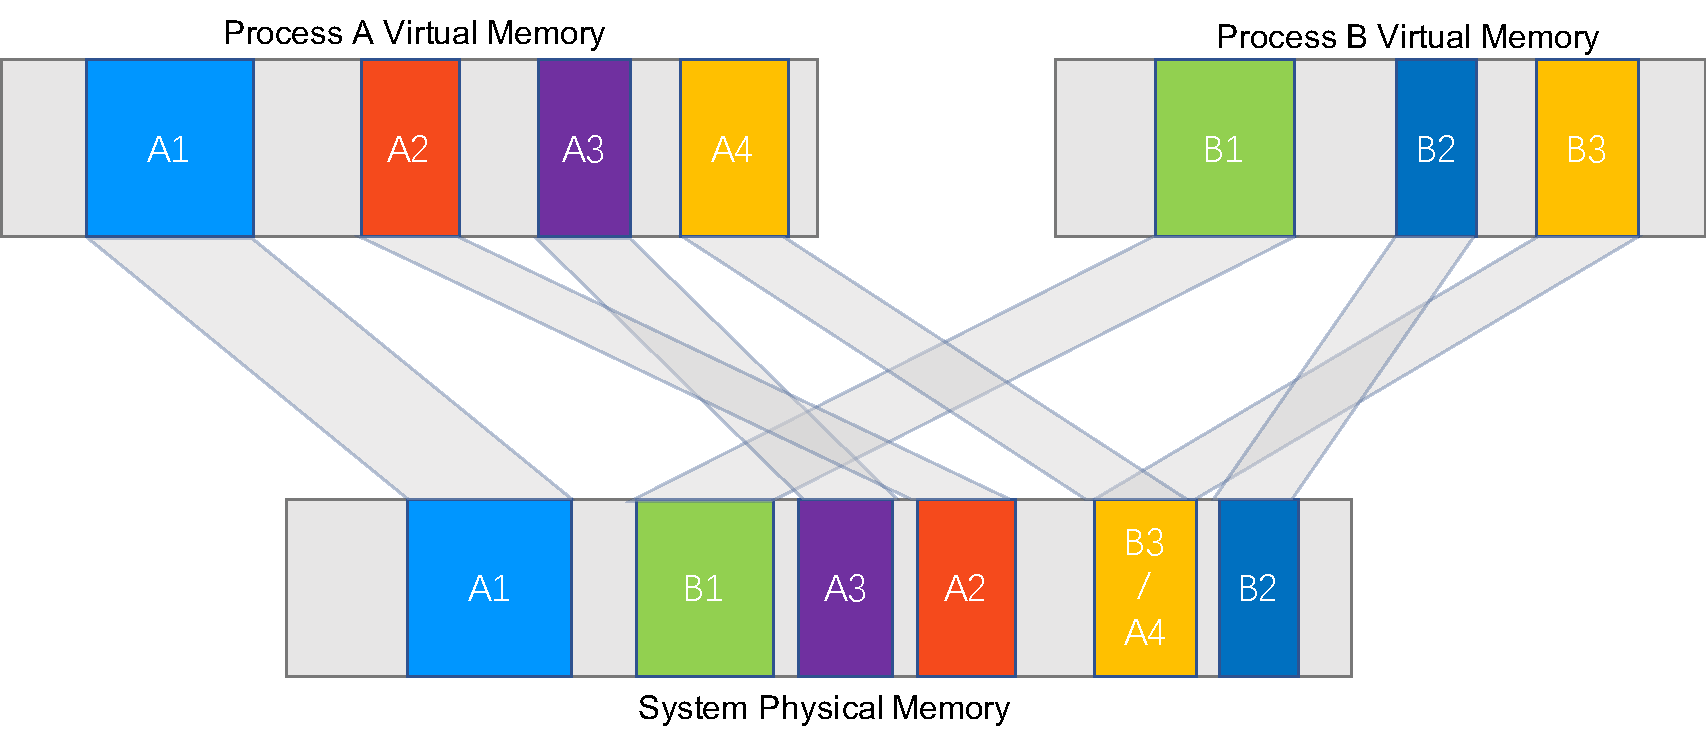
\includegraphics[width=12cm]{memory.pdf}
  \bicaption[Linux虚拟内存映射原理]
    {Linux虚拟内存映射原理}
    {Mechanism of Linux Virtual Memory Mapping}
  \label{fig:MEM}
\end{figure}
由此可见,物理内存页的状态分为三种:没有被映射到任何进程的虚拟内存里(未使用的物理内存页),被映射到唯一的线程的虚拟地址空间里(例如线程的用户栈),被多个进程共享(如共享库);而所有的虚拟页也分为三种:未被映射的虚拟内存页,映射到独占的物理内存的虚拟内存页,以及映射到共享内存的虚拟内存页。如图\ref{fig:MEM}所示,进程A、B的虚拟内存由已映射物理内存的页和未映射物理内存的页组成,其中A1、A2、A3物理页由进程A独占,B1、B2物理页由进程B独占,A4和B3物理页被同时映射到进程A和B的虚拟地址空间中。只要A进程和B进程中的一者对A4(B3)虚拟内存区域作出写操作,另外一个线程即可读到该写操作的内容。而在不共享物理页面的虚拟内存区域进行写操作,则不反映到另一个进程的虚拟地址空间里。这个同步过程是由硬件的缓存一致性机制(cache coherent mechanism)所保证的,当这两个进程中的一者写入后,另一者再次对该区域的内存进行访问,则会引起cache miss(缓存不命中),于是可以读取到内存中最新的内容。

\subsection{非一致性内存访问架构}
历史上,为了提高系统的计算能力,一开始是通过加快CPU的运行频率,直到CPU频率的提高遇到了瓶颈,硬件设计者就设计了多核CPU。越来越多的CPU核通过系统中唯一的北桥来读取内存(这种架构被称为一致性内存访问架构,UMA),当CPU核的数量多到一定程度时,各个CPU核之间对北桥的竞争越来越激烈,内存访问的延迟越来越大,使得北桥(具体来说,是北桥上的集成内存控制器,IMC,Intergrated memory controller)成为计算机性能提升的新的瓶颈。于是硬件设计师将所有的CPU分组,每个Socket上的CPU为一组,系统中有多个Socket。每个socket上的CPU是一个NUMA节点,并且给每个CPU小组分配独立的内存,称作本地内存。每组的CPU在同一个Socket上,共用同一个集成内存控制器,竞争北桥的CPU数量就得到了明显下降,CPU访问本地内存(local access)的速度得到了提高。然而,只有在CPU访问本地内存时延时较短,而访问其他NUMA节点的内存(remote access)就需要经过QPI Interconnect通道,增加了访问时延,故得名NUMA。
\label{chap:memm}
Linux内核使用Node(节点)、Zone(区)、Page(页)三级结构描述物理内存\cite{phymem}。对于UMA架构,内核中只存在一个静态Node结构,而对于NUMA架构,内核可以自由增删Node结构,用Node结构体管理一个NUMA节点的本地内存。每个Zone用于不同的功能,而Page是内存与磁盘交换数据的单位。当Linux进程申请物理内存时,内核优先将本地节点的物理内存分配给这个进程,如果仍未满足需求,则向临近的NUMA节点请求内存页,最终满足内存需求。Linux调度器对NUMA架构做了优化,即当调度发生时,优先选择本地节点上的进程调度。如果本地节点的资源使用率超过了一个界限,则触发负载均衡机制,将该进程从本地节点移动到最合适的节点上。Linux的内存映射机制也对NUMA架构进行了优化。Redhat公司的Rik van Riel提出了Automatic NUMA Balancing(NUMA自动平衡)机制\cite{balancing},经过一段时间(Scan delay)扫描进程的地址空间,将进程虚拟地址空间中的一小部分页面\footnote{一般是256MB}取消映射(unmap)。当进程对这些被unmap的页面进行访问时,会触发NUMA page fault(NUMA缺页异常)。Numa Page Fault向操作系统报告发生page fault的页面的位置,从而得出该进程使用的页面在NUMA系统中分布的位置,从而将进程移动到内存访问最多的节点上。

经过硬件工程师和软件工程师的共同努力,单个服务器装备的CPU数量得到了巨大的提升,单个程序也很难将整个机器跑满,从而促进了云的发展,将海量的物理资源通过虚拟机、容器等形式分发给数量众多的用户,开启了云时代。本文中,巨型虚拟机为客户机提供的是一个NUMA架构的系统,而分布式共享内存(DSM)的性能特性和NUMA架构类似,故针对NUMA架构的优化也可以使用在巨型虚拟机上。
\section{巨型虚拟机架构简述}
\subsection{系统虚拟化简介}
在计算机科学中,增添抽象层次是一个很重要的研究方法。在不同的场景下添加不同的抽象层,得到的结果大不相同。如果将抽象层置于CPU上,则会产生进程的概念,为系统中所有的任务\footnote{Linux将线程和进程都称为任务,task\_struct,不做特殊区分}抽象出可以独占的CPU,从而让CPU被分时复用,从而使得其性能得到最大化的利用。如果将该抽象层置于物理内存之上,则产生虚拟内存的概念,使得进程获得了一个连续的广阔的虚拟地址空间。如果抽象出一个ISA(Instruction set architecture,指令集架构),即一个计算机运行的硬件环境,则是虚拟化(system virtualization)这一重要概念。VMM(虚拟机管理器)可将客户机运行在虚拟的硬件之上,系统虚拟化将操作系统与底层硬件解偶,具有诸多的优势,例如良好的封装性、硬件无关性\cite{sysv},这使得虚拟机可以在任何时候停止执行,通过快照在任何时间恢复先前的执行,方便了虚拟机的迁移与容错,促进数据中心的负载均衡。本文正是利用了虚拟化这个抽象层的这一优点。

历史上,纯软件虚拟化技术的出现早于硬件辅助的虚拟化技术。早期的二进制翻译技术(即将每条客户机指令在执行时进行翻译,类似于解释型编程语言),是完全基于软件的虚拟化。由于软件模拟硬件行为的复杂性,纯软件的虚拟机监控器工程量巨大,代码复杂,同时模拟出的虚拟硬件性能相比于真实硬件有明显下降。之后出现了半虚拟化(Para-Virtualization)技术来弥补纯软件虚拟化方式的不足。其想法是为虚拟机管理器定制客户机OS,使得客户机明确地知晓自己处在虚拟化环境中,与虚拟机管理器相互配合,解决了体系结构造成的虚拟化漏洞。最具有代表性的基于半虚拟化的虚拟机监控器就是Xen\cite{artofxen},Xen运行的定制的guest OS调用Xen的接口配合Xen完成虚拟化功能。但是,由于Windows等闭源操作系统的存在,半虚拟化的可应用范围依然受限。现如今,硬件辅助的虚拟化是应用最为广泛的虚拟化方式。Intel推出的VT-x(Virtualization Technology for x86 processors)技术\cite{intelv}和AMD推出的SVM(Secure Virtual Machine Architecture)技术\cite{amdv}在现有的CPU指令集架构上增加了专用于系统虚拟化的指令,例如Intel的VMX指令(有VMPTRLD、VMREAD、VMWTRITE等)\cite{intelSDM}。x86架构的处理器有根与非根两种运行模式,客户机运行在非根模式,当客户机的特权指令执行时,将触发VMexit,于是CPU运行模式自动转换,使得VMM可以通过trap-and-emulate(陷入并模拟)方式模拟客户机的特权指令。硬件辅助的优点是免去了客户机的修改;又由于客户机指令无需翻译,便可以直接运行在真实的硬件CPU上,使得CPU虚拟化的代价也大大减小。

对于内存虚拟化,传统的方式是为每一个客户机进程维护一个shadow page table(SPT,称为影子页表),代替客户机自带的页表,将其覆盖(shadow),每当进程修改GPT,就需要对SPT进行维护。然而当客户机进程数量较大时,影子页表维护和保存的开销将会十分可观。同时,由于客户机修改自己的页表(GPT)时SPT也要进行相应的修改,VMM将GPT所占的内存标记为写保护(write protected),当客户机修改GPT时会引起VMexit,退出到VMM中由VMM完成对SPT的维护。这对于memory intensive(内存密集)型任务是一种灾难,因为会引起大量的VMexit,严重影响其性能。硬件机制EPT(Extended Page Table)使用硬件维护的GPA到HPA的映射,替代了软件实现的SPT。客户机依然使用自己的CR3指针进行地址翻译,将GVA翻译为GPA,而每一个guest OS都有其对应的扩展页表,EPT base pointer(扩展页表基指针)指向扩展页表(EPT),将GPA通过硬件翻译为HPA。于是,客户机修改自身的GPT(guest page table)时无需引起VMexit,提高了性能。硬件上也有类似于传统页表TLB(translation look aside buffer)的应用于EPT的页表,缓存了EPTE(EPT表项),加快了由GPA到HPA的翻译。使用本文所使用的巨型虚拟机即利用了这一硬件扩展,实现了内存的高效虚拟化。

VMM又可分为Type-\uppercase\expandafter{\romannumeral1}型和Type-\uppercase\expandafter{\romannumeral2}型。Type-\uppercase\expandafter{\romannumeral1}型又称为Hypervisor型,直接运行在裸金属上,全权负责虚拟机的创建、调度、运行、电源管理等,是一个完备的操作系统,所以需要编写大量驱动以及操作系统功能,工程量较大,但也具有更好的性能。而Type-\uppercase\expandafter{\romannumeral2}型VMM事实上是host OS的一部分(内核模块),仅仅具有虚拟化的功能,而最基本的操作系统功能由host OS负责完成。还有混合型虚拟机监控器,它同样运行在裸金属上,但是将设备驱动、设备模型的控制权交由一个特权虚拟机。Xen属于混合性虚拟机,它将操作系统应当实现的功能交由domain 0这一特权操作系统完成。然而,Type-\uppercase\expandafter{\romannumeral1}型和混合型虚拟机需要修改客户机操作系统,这对闭源操作系统是不现实的,同时减小了虚拟化的灵活性,故没有得到大范围应用。而开源虚拟机监控器QEMU-KVM属于Type-\uppercase\expandafter{\romannumeral2}型,KVM\cite{KVM}是Linux内核中安装的kernel module(Linux内核模块),而QEMU\cite{QEMU}是运行于用户态的宿主机应用程序,主要负责应对客户机的I/O请求,将KVM作为其虚拟化加速器,KVM利用x86处理器的VT-x、EPT等硬件辅助虚拟化功能获得了更优的虚拟机执行效率,而无需修改客户机操作系统,得到了广泛的应用。下一节中的巨型虚拟机即通过修改QEMU-KVM这一开源虚拟机监控器得以实现。
\subsection{巨型虚拟机架构实现}
巨型虚拟机属于分布式虚拟机,即把一个分布式系统作为运行的物理基础,对上层提供统一的操作系统接口。其主要目的是为了资源聚合,即将分布式系统中的多个普通单机聚合起来,形成一个纵向扩展的虚拟机。例如,普通计算机的CPU核心数目一般在50以内,而更多CPU核心数目的机器则会非常昂贵\footnote{36个CPU核心是服务器较为典型的配置。详见 https://www.quora.com/What-are-the-specs-of-a-typical-modern-server}。有了巨型虚拟机,我们可以将多个普通且廉价的物理机聚合起来,启动一个拥有海量资源的虚拟机,例如将5个配备36个CPU的服务器进行资源聚集,我们可以得到一个拥有180个虚拟CPU的客户机,这是单个物理机很难达到的配置,同时具有了纵向扩展系统和横向扩展系统的优势。

巨型虚拟机基于QEMU-KVM这一Type-\uppercase\expandafter{\romannumeral2}型虚拟机监控器(修改后的QEMU称作dQEMU,distributed\,QEMU),将QEMU-KVM扩展为分布式虚拟机。其实现主要分为三个部分,这与系统虚拟化常见的三个需要完成的部分相同:实现分布式vCPU、分布式虚拟内存,以及分布式虚拟I/O。支持巨型虚拟机运行的物理基础是多个物理机组成的集群,在集群的每个节点上,都运行着一个巨型虚拟机的dQEMU实例。每个实例都拥有整个集群的资源,但是属于本机的资源标记为local(本地资源),而集群中其他节点的资源标记为remote(远程资源)。当本地虚拟机实例对远程资源发起请求的时候,路由模块会找到所访问资源的真实位置,将资源请求转发到真正拥有该资源的节点上。而内存资源是一个例外:所有的虚拟机的QEMU实例拥有全部的内存资源,由DSM(distributed shared memory)进行提供。完成分布式虚拟化的三个主要功能模块有:


\noindent\textbf{分布式vCPU}\quad 巨型虚拟机添加了新的QEMU参数,将一部分本地运行的vCPU标记为local vCPU,而其他未标记的vCPU则是remote vCPU。QEMU为所有的vCPU创建APIC。local vCPU线程在完成初始化之后可以继续执行,而remote vCPU线程初始化完成后阻塞(被调度器放置于睡眠队列),直到虚拟机被销毁。当有IPI(inter processor interrupt,处理器间中断)发送给vCPU时,会向目标APIC的APIC ID寄存器、LDR(Logical Destination Register)寄存器、DFR(Destination Format Register)寄存器写入IPI请求。远端vCPU的APIC称为dummy APIC(傀儡APIC)。dQEMU为每个vCPU在其本地QEMU实例上维护一个真实APIC,而在其他的所有QEMU实例上维护一个dummy APIC。在写入请求时,检查该IPI是否发送给远程vCPU,即检查上述三个寄存器的写入是否是对dummy APIC进行写入。如果是发送给本地vCPU,即向真实APIC写入,则按照原有流程处理;否则,该QEMU实例将对IPI请求进行转发,将IPI注入到远程APIC,同时将集群中所有该vCPU的APIC拷贝强制同步,由远程的QEMU实例接收IPI请求并进行处理。如果集群中有四个节点,每个节点分别运行QEMU 0-3,而每个QEMU实例分别有vCPU 0-3。当vCPU 0向vCPU 3发送中断时,先向QEMU 0中vCPU 3的dummy APIC写入上述三个寄存器,同时QEMU 1-3从QEMU 0得到最新的APIC状态。QEMU 3通过APIC识别出vCPU 3是IPI的接收者,故QEMU 3将IPI注入到vCPU 3。

\noindent\textbf{分布式共享内存}\quad 内存虚拟化模块是巨型虚拟机最关键的部件,为所有的QEMU实例提供了和普通内存完全相同的接口,使得所有虚拟机共享完全相同的虚拟地址空间。普通QEMU为虚拟机分配内存的原理是,通过执行一次mmap()函数,在宿主机虚拟地址空间中分配guest OS物理内存。在分布式共享内存开发的初期,为了尽早测试分布式共享内存的代码,巨型虚拟机在单机上进行测试,将所有QEMU实例的虚拟机内存映射到同一块内存,即对相同的文件调用mmap()函数,从而使得所有QEMU实例拥有共享的内存空间。在开发的后期,在KVM中实现了DSM模块,并与QEMU对接,才转向真正分布式的DSM实现,即通过RDMA或TCP协议进行所有QEMU实例之间内存的同步。

如图\ref{fig:DSM}所示,分布式共享内存(DSM)主要通过维护EPT中页表项的状态,即维护虚拟机所拥有物理内存页的状态,修改EPT的映射,将客户机的物理内存映射到集群中的各个节点。DSM的设计基于Ivy\cite{ivy},Ivy实现了MSI protocol,满足了SC(sequential consistency,顺序一致性)。每个客户机物理页的状态分为Modified:本地vCPU对页作出修改,远程vCPU尚未获得该页的修改,Shared:本地vCPU和远程多个vCPU共享该页,Invalid:需要向其他节点获取该页的最新拷贝,否则本地vCPU无权对该页进行读写。所以,在某个dQEMU实例触发Page fault时,需要使用RDMA协议或TCP协议向远程节点请求最新的数据页。由于巨型虚拟机中的分布式共享内存需要至少实现x86-TSO(Total Store Order)\cite{tso}弱的内存模型,故节点间内存同步的次数和较弱的内存一致性模型相比更多。如果巨型虚拟机的两个节点上的进程相互共享过多的内存,势必会增加内存同步的开销。分析并减小这类开销是本文关注的重点之一。
\label{chap:DSM}
\begin{figure}[!htp]
  \centering
  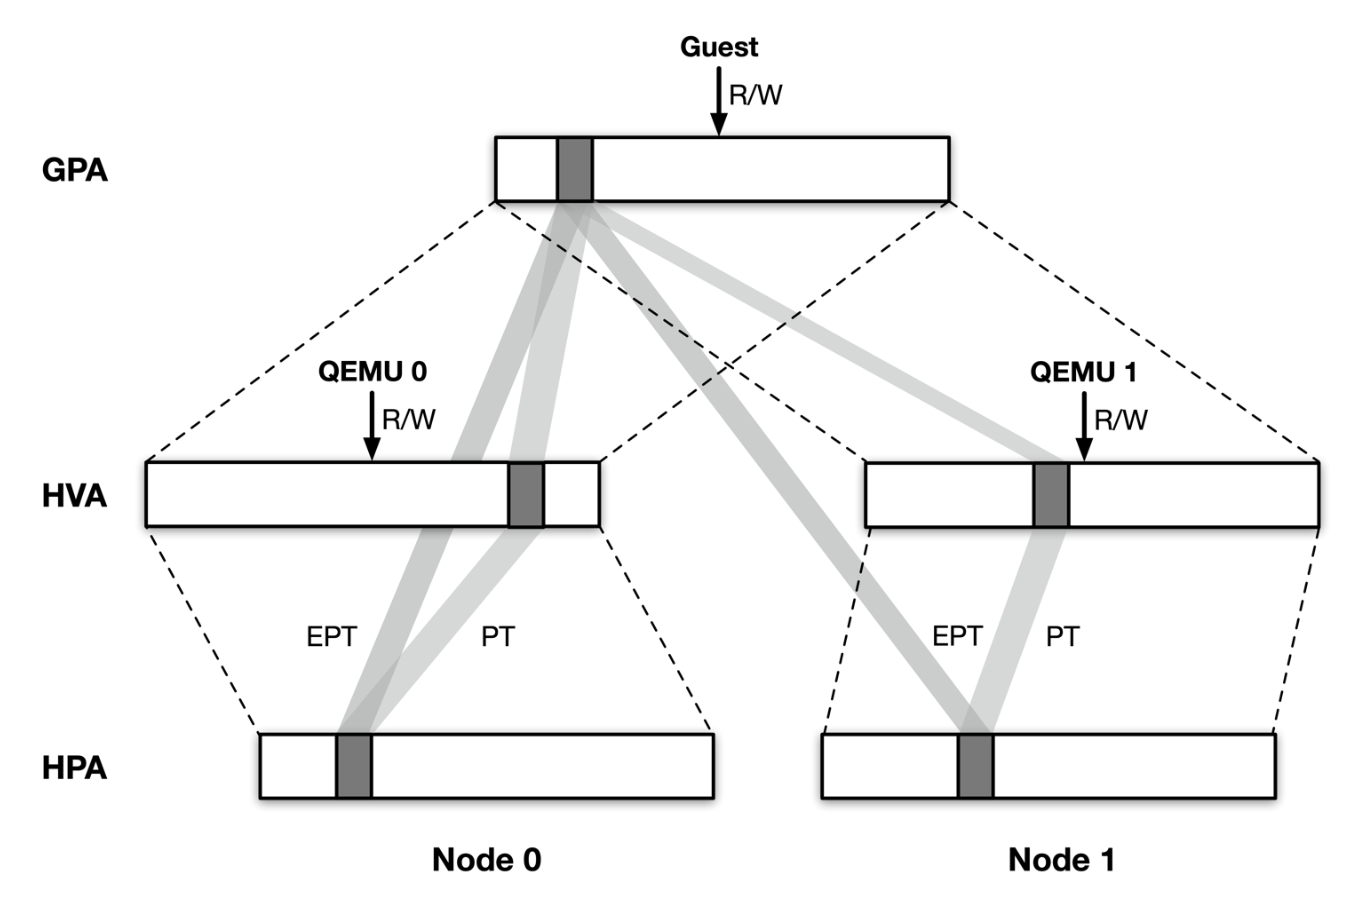
\includegraphics[width=10cm]{dsm.png}
  \bicaption[巨型虚拟机的内存映射]
    {巨型虚拟机的内存映射\cite{giantvm}}
    {Memory Mapping of Giant Virtual Machine}
  \label{fig:DSM}
\end{figure}

\noindent\textbf{I / O虚拟化}\quad 实现分布式虚拟I/O需要解决以下问题:虚拟机vCPU如何对远程节点上的的模拟设备进行I/O访问,以及如何使得远程的虚拟设备产生的中断准确的路由到对应的vCPU。对于第二个问题,分布式vCPU的虚拟化中对于IPI的处理已经给出了答案,即在QEMU 0上放置master IOAPIC,而在QEMU 1-3上放置dummy IOAPIC。在设备中断到达之后写入dummy IOAPIC时,将信息同步至master IOAPIC,由master IOAPIC将中断通过dummy APIC转发给目的vCPU。对于第一个问题,CPU对设备进行I/O访问有两种方式:PIO(Programmed I/O,针对于x86架构)和MMIO(Memory Mapped I/O)。客户机执行I/O指令后退出到VMM,VMM检查I/O指令的目的设备。如果I/O访问的目的设备是远程机器上的设备,则需要将该请求转发给远程设备,在处理完成后将处理结果发送回来。目前,巨型虚拟机的模拟设备全部放置在master node上。

\section{分布式共享内存性能分析}
\subsection{性能瓶颈}
\label{chap:bottle}
如\ref{chap:DSM}节所述,巨型虚拟机相比于普通虚拟机的实现增加的部分有:(1)分布式共享内存,这一部分需要通过RDMA、TCP等网络协议在集群之间同步物理页的状态;(2)转发机制,将对于远程资源的访问请求转发到对应的节点上去,由真实的资源拥有者处理访问请求。这两部分均会产生网络开销,而网络开销最大的则是分布式共享内存这一组件。由于顺序一致性是是较强的一致性模型,分布式共享内存会产生false sharing(伪共享)现象和page thrashing(页面颠簸)现象\cite{sharing}。伪共享现象是指两个运行在不同CPU核心上的线程不断地写入同一个cache line(缓存行)中的变量,当其中一个线程对变量写入后,另一个核上的缓存行即会失效,于是另一个线程需要从内存中读取最新的数据,而写入变量的线程也需要将缓存行写回主存。如此循环往复即出现了伪共享现象。而页面颠簸现象是由于内存页的换入换出。当一个进程频繁访问的页面数量多于总的物理页面数量,或者操作系统为进程选取的驻留集大小(RSS,可以通过ps aux等命令行工具观察进程的驻留集大小)小于其频繁访问的虚拟空间大小,则会有虚拟页面不断换出到磁盘上,即产生了页面抖动现象。

\label{chap:STOR}
伪共享现象和页面抖动现象都是因为不同层次的存储器访问延迟大不相同造成的。现代计算机有如下几个存储器层次\cite{csapp}:
\begin{itemize}
  \item L0 寄存器:在CPU内部用来存储指令和数据。访问时间不超过一个CPU cycle(CPU时钟周期),用于缓存来自高速缓存(L1-L3)的数据
  \item L1-L3 高速缓存(SRAM):静态RAM,L1访问需要几个时钟周期(约为4个时钟周期),L2访问需要几十个时钟周期(约为10个时钟周期),L3访问需要近百个时钟周期(约为40个)\footnote{数据来源:https://v2ex.com/t/523069}。L1分为数据缓存(dcache)和指令缓存(icache),L1、L2由单个CPU核独享,L3由处理器中所有的核共享,保存来自于L4的数据。
  \item L4 主存(DRAM):动态RAM,访问需要几百个时钟周期(100ns),用来缓存来自磁盘的数据。
  \item L5 本地的二级存储,即磁盘(Disk):磁盘分为SSD(固态硬盘)和HDD(机械硬盘),SSD一次读取时间为16,000纳秒,HDD一次读取时间为2,000,000纳秒。
  \item L6 远程二级存储(Web服务器等):经过网络协议与网络进行数据交换,访问时间约为150,000,000纳秒\footnote{数据来源:https://stackoverflow.com/questions/4087280/approximate-cost-to-access-various-caches-and-main-memory}。
\end{itemize}

为了获得更大的容量,则会遭受更高的延迟。由于分布式共享内存增加了物理内存的容量,需要通过网络访问远程节点的内存,相比于本地内存访问增加了网络开销,所以成为了性能瓶颈。如果在不同节点上的应用程序频繁访问共享的地址空间(如内存密集型任务、I/O密集型任务),则需要分布式共享内存模块进行大量的内存同步工作,不仅造成客户机内存访问的延迟明显提高,使得巨型虚拟机可扩展性降低,还会占用集群中宝贵的网络带宽。虽然分布式共享内存模块已经利用RDMA、压缩优化等技术大大减小了其占用的网络带宽,但仍需要解决根本问题,对巨型虚拟机的客户机调度器进行重新设计,使得节点间访问共享内存的机会更少,增强客户机内存访问的局部性。
\subsection{增强访存局部性的方式}
由\ref{chap:mem}节和\ref{chap:memm}节所述,造成进程之间频繁访问共享内存的原因之一是共享的内核数据和代码。由于对内核数据结构的频繁访问,硬件为了保持缓存一致性,会频繁的从内存中读写数据,造成如上节所属的分布式共享内存所遇到的两个问题。于是,来自ETH Zurich的研究者们从操作系统的内核架构开刀,将宏内核切分开来,实现了一个多内核操作系统Barrelfish\cite{barrelfish}。Barrelfish操作系统将现代的计算机系统视作一个网络,每一个CPU核以及它所附带的缓存是该网络中的一个节点。其设计理念有如下三点:

\begin{figure}[!htp]
  \centering
  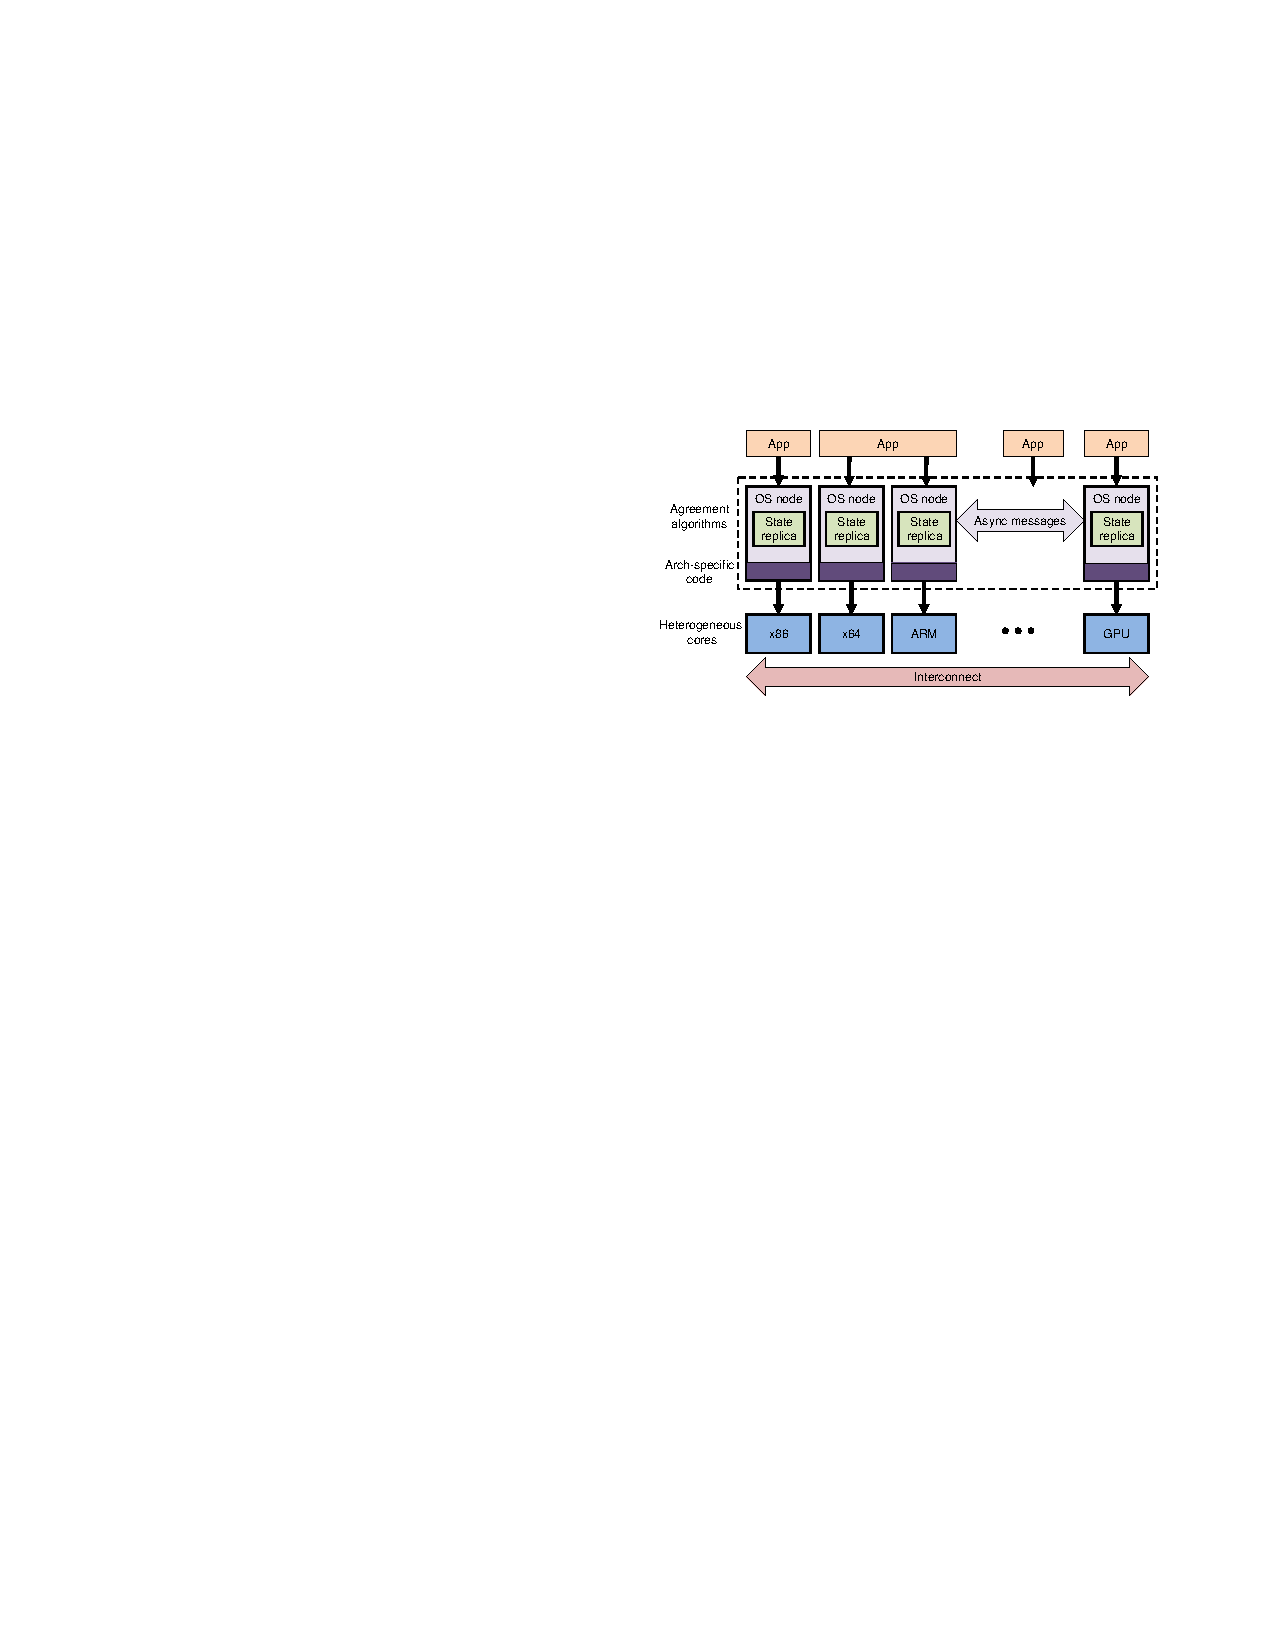
\includegraphics[width=12cm]{barrelfish_sosp09.pdf}
  \bicaption[Barrelfish OS多内核架构]
    {Barrelfish OS多内核架构\cite{barrelfish}}
    {Architecture of Barrelfish OS Multikernel}
  \label{fig:barrelfish}
\end{figure}

\noindent\textbf{核间显式通信}\quad 在宏内核的操作系统中,CPU核与CPU核之间的通信大量依赖于共享内存。然而,如果将单个计算机的硬件视作分布式系统的话,那么将共享内存(shared memory)作为通信的渠道将获得类似于广播的效果:只要映射了这块物理内存的所有进程将会收到这条信息。所以,发送一条信息耗费的时间将会随着硬件系统中的节点数成正比地增加。这是由于CPU在等待缓存一致性机制完成数据同步,从缓存不命中中返回于是发送一条信息的时间也会随着信息量的大小而线性增长。而在消息传递(message passing)模型中,存在服务端线程(server thread)和客户端线程(client thread),服务端线程固定地运行在一个CPU核上,维持着所有客户端线程所需的信息。所有客户端线程只需发送一个远程过程调用(RPC, remote procedure call),虽然远程过程调用所传递的信息依然通过共享内存进行传递,但只是控制面的信息,而真正的数据一直保持在服务端线程的缓存中,不会出现缓存不命中的现象。核与核之间的通信在宏内核中不是显式的,而是隐式的通过共享内存来进行,这样会造成大量不必要的开销。而在Barrelfish操作系统中,核与核之间的通信仅有远程过程调用,而不存在其他类型的通信。故Barrelfish操作系统具有良好的内存访问局部性。

\noindent\textbf{操作系统内核与硬件解耦}\quad 这部分设计理念将操作系统内核的通信算法(策略,policy)与硬件相关的通信机制优化(机制,mechanism)进行解耦合,降低工程量。这不在本文的讨论范围内。

\noindent\textbf{全局状态分散为多个副本}\quad 操作系统经常维护一些全局状态,如Linux内核中的runqueue(就绪队列)。当多核时代来临之后,就必须用锁来同步。为了避免锁的开销,常用的办法是将全局状态分解到每一个CPU核上,在Linux 2.4版本\cite{linux}中引入了per-CPU runqueue,极大的提升了调度器的可扩展性,达到了O(1)的运行时间,即调度器运行时间和系统中CPU核的数量无关。在Barrelfish操作系统中,这个概念更进了一步:将所有的内核状态分散在各个CPU核上。如图\ref{fig:barrelfish}所示,内核状态分散在各个CPU核上,只在必要时进行同步。


Barrelfish OS较少的核间通信使得其成为了巨型虚拟机理想的客户机操作系统。即使是如I/O密集型的大量访问内核数据结构的任务运行在Barrelfish客户机中,分布式共享内存也应该具有很好的扩展性。我们分别在Linux和Barrelfish上运行了WebServer,Linux的WebServer是Apache2,而Barrelfish OS的Webserver是调用了Barrelfish操作系统接口的Webserver,所以减少了大量不必要的核间通信。使用ab(ApacheBench)\cite{ab}这一测试工具不断地向WebServer发送GET请求,Barrelfish OS上运行的WebServer比Linux中的WebServer处理速度快6.4倍\cite{giantvm}。这是由于Barrelfish OS大大限制了核间通信的次数和传递的信息量,将所有的核间通信限制在RPC中,分布式共享内存发生缺页异常的次数也得到了限制,减小了网络开销。
\section{数据中心及其资源利用率}
数据中心(Internet Data Center)为内容提供商、企业、政府部门等需要对数据进行保存、共享、操作的组织提供了一个高效安全稳定的运行环境。数据中心由数量巨大(成百上千)个服务器组成,每个服务器称作该集群中的一个节点,每个节点之间通过高速的网卡进行连接,同时为其提供稳定的电力供应、温控、及时维护等服务,目的是使得数据中心对外提供高质量、稳定的服务。数据中心的搭建还要考虑成本问题,如果将数据中心搭建在气温较低的环境下,则会为数据中心运营者减少很多散热的成本;CPU也为使用者定义了ACPI(Advanced Configuration and Power Interface,高级电源管理接口,其中规范了G-States、S-States、C-States,可以通过调整CPU和整个系统所处的等级来应对不同要求的任务)规范,给软件编写者一个动态调整CPU功耗的方式,从而充分利用CPU,减少功耗成本。而数据中心的资源利用率问题则是数据中心运营者所考虑的关键:如果提高了资源利用率,则意味着可以通过更少的机器对外提供相同质量的服务,同理也意味着可以使用相同的机器提供质量更好、数量更多的服务(例如更高的吞吐量),从而在节约成本的同时,获取更多的效益。提高数据中心资源使用率在一定程度上等同于数据中心的负载均衡:将负载过重的机器上的工作负载迁移到较空闲的机器上,提高了系统总体的并行度,也提高了系统的资源利用率,一些负载均衡的方法也可以达到提高资源使用率的效果。

本文使用基尼系数(Gini Coefficient)\cite{gini}衡量集群CPU资源使用率的均衡情况。基尼系数普遍用于计量经济学,用来表征居民收入的不平均程度。基尼系数是0到1之间的一个数,对于一组完全相同的数据,其基尼系数为0,即最平均;低于0.2则意味着这组数据高度平均,在0.2-0.29之间表示比较平均,0.3-0.39之间表明平均程度一般,0.4-0.59之间则表示同组之间数据差距较大,而在0.6以上则表明这组数据极为不平均。一组全部为1的数据的基尼系数为0,而对于一组均匀分布在0和1之间的数据,其基尼系数为0.333(三分之一),对于有一千个0和一个1的数据,其基尼系数接近于1。我们将其应用在分析数据中心的CPU占用率上,我们认为集群总体的CPU资源占用率的基尼系数在0.25以下表明该集群的负载比较均衡,资源使用率也较高。

历史上,提高数据中心资源利用率的方式有如下三种:

(1)任务混部:这是最符合直觉的一种提高资源利用率的方式,即将更多的任务放在同一个资源较为充裕的机器(或几个机器)中,这样必然使得固定数额的资源得到更好的利用。但是这会对被混部在一起的任务造成影响,由于对资源的更加强烈的竞争,某些获得不到充足资源的任务的服务质量将无法达到预期程度,即服务质量遭到破,又称QoS\,violation。由于任务的多样性及其工作负载的多变性,资源控制器不能及时地调整任务的混部情况;即使在同一个节点上有很多方式限制一个进程的资源使用量(如cgroup,一种限制单个进程或一组进程的资源使用量的机制),但这依然无法实时地保证各个进程获得了充足的资源。

(2)工作负载即时采样:通过硬件或者软件的手段对任务的资源占用情况进行即时的采样,根据任务在过去一段时间里的工作负载情况预测未来一段时间内的工作负载情况。例如,最常用的Linux内核所实现的完全公平调度器(CFS,Completely Fair Scheduler)即是采用了这一种策略:在内核表示任务的结构体struct task\_struct中内嵌(由于struct sched\_entity内嵌在struct task\_struct中)一个vruntime变量,记录其已经运行的时间,在每一个调度周期中更新这个变量。每个CPU上的就绪队列维护了一个红黑树,每当一个进程变成可运行状态(RUNNABLE)时将进程按照vruntime添加进入红黑树中,而Linux内核通过vruntime判断在未来一段时间内该进程的运行时间。然而,这样的预测不一定完全准确,甚至有的时候出现完全的预测错误。同时,取样的数据也不一定具有代表性。

\label{chap:reallocation}
(3)资源重分配:为了解决集群中工作负载分布不均的问题,一种更加灵活的方式是将任务在不同的节点上迁移,将资源在任务之间重新分配。迁移的具体方式有进程级别的迁移(Process Migration)、容器的在线迁移(Container Live Migration),和虚拟机的在线迁移(VM Live Migration)。这类似于任务调度,但发生在集群中的节点之间,用于平衡集群中节点的负载,进而提高集群的资源使用率。在下面的三节中,我们将对这三类迁移机制进行详细的描述,并且讨论其优劣。
\subsection{进程迁移}
进程级别的迁移主要具有两方面的作用,性能提升和容错\cite{processmigration}。首先是可以得到性能上的提升,进程从较为繁忙的处理器上重新分布到较为空闲的处理器上,使得处理器的负载尽可能均衡,从而提高了系统中进程的并行度和处理器的平均使用率。同时,进程访问物理上较远处的资源会造成更大的通讯开销,例如在非一致性内存访问系统中,访问远程NUMA节点的内存比访问本地内存的开销要大得多,所以Linux内核为适应NUMA架构则将进程迁移到其所访问的内存所在的节点上。其次,进程迁移有助于提高大型系统中的错误包容(Fault Tolerance, FT)能力。现今的大规模分布式任务可同时使用的处理器个数已经成千上万,在如此庞大的系统中,出现CPU核、内存、网卡、磁盘等部件崩溃的情况越来越多。数据的可靠性可以通过增加副本的方式解决,但会占用额外的资源。进程级迁移为容错提供了一个新的选项,即可以以一种对软件透明的方式,把遇到硬件崩溃的进程停止,为其进行快照,保存其运行状态,迁移到硬件可以正常工作的环境下恢复进程的执行。进程调度由进程管理线程或由进程自身发起。当该管理线程探测到某些进程满足了迁移的条件,如主机的负载过高,则向操作系统内核发起一个进程迁移请求,于是被迁移的进程被标记为In Migration,并将其移出runqueue,但其运行状态不被改变,由于其到达目的主机之后的进程状态应当不被改变。当源主机做好迁移准备后,即向目标主机内核发送一个信息,请求线程的移入,请求附带的信息有进程的资源占用情况和运行状态等。如果目标主机可以接收该进程,则为该进程分配资源。完成分配后,即将源主机上的进程状态复制到目标主机上,同时复制其他进程资源。拷贝完成后,源主机将所有发向该进程的信息转发给目标主机,并等待目标主机上的进程重新恢复执行。最后的任务包括释放源主机上的进程资源,以及恢复目标主机上进程的执行。为了提高进程迁移的效率,有不同的算法被先后提出\cite{migrationppt}。如Lazy copy(延迟拷贝)算法,将被迁移进程从源主机的运行队列里移除之后,首先传输进程在目标主机上执行所需的最小信息,使得进程的In Migration时间缩到最短。但是由于未迁移的状态仍保留在源主机上,如果源主机在进程迁移的过程中崩溃,则被迁移的进程所拥有的信息会遭到丢失,增加了进程的不可靠性。同时,打开的文件、共享内存和发送的信息等资源作为进程间通讯的手段,改变了进程通信的愿有语义,会给被迁移进程带来残余依赖性问题。故进程迁移没有被工业界大规模使用,应用程序也很少有对进程迁移的适配。
\subsection{容器热迁移}
\label{chap:containermigration}
容器(container)\cite{container}的出现最初是为了解决应用程序配置部署环境的问题。容器技术将应用程序的运行环境与应用程序本身绑定,将应用程序和其运行环境打包为一个独立的容器镜像,在任何环境下无需重复配置环境即可部署。容器技术同时解决了上述的残余依赖问题,将进程运行在一个具有所有其运行所需的最小资源环境里,与其他进程使用的资源隔离。容器技术因为其轻量、标准化、安全性高等特点,受到微服务(MicroService)架构的青睐。容器相比于虚拟机的启动时间小、内存足迹(memory footprint)小、迁移的网络开销小,可以在同一台服务器上部署成千上万的容器,而虚拟机则拥有整个操作系统的信息,单台机器上无法做到高密度的部署。事实上,一个容器实例是Linux系统中的一个进程,只是和普通的进程相比增加了Namespace、cgroups等运行参数,取消了进程层面上的共享,把残余依赖限制在同一个容器实例中。容器的热迁移\cite{Voyager}具有和进程迁移相似的作用:负载均衡和容错。对于容器迁移的优化目标是缩短Downtime(下线时间),尽可能地减小对服务质量的影响。

内存状态的迁移是容器迁移的主要内容,目前有两种内存的迁移策略:precopy(前拷贝)和postcopy(后拷贝)。对于前拷贝,内存页的拷贝发生在容器迁移之前,即发起迁移请求后,容器继续在源节点上运行,而容器的内存页已经开始向目的节点迁移。在每一轮的内存页拷贝中,不断的有上一轮拷贝至目的节点的内存页被容器修改,所以在本轮中重新传输。在经过一定数量的拷贝次数之后,迁移管理进程发现将拷贝循环继续进行下去将很难把所有内存拷贝到目的节点,此时容器冻结(freeze,停止运行),将所有内存页拷贝至目的节点,并恢复容器的执行。由于这一前拷贝过程中内存页被不断地修改,所以对容器中内存密集型的任务不友好,会产生大量的网络开销。因为容器冻结后被修改的内存页数量比所有的内存页一般更少,所以这一迁移方式的下线时间更短。对于后拷贝,拷贝过程一开始就将容器冻结,并将容器的处理器、寄存器、设备等最小执行状态发送给目的节点,而不发送数据量较大的内存状态,使得容器以最短的下线时间开始执行。然而在目的节点开始执行后,容器会产生大量的远程缺页异常(remote page fault),也要等待远程内存页在网络上的传输,导致容器在新节点上开始执行之后的效率十分低下。这种迁移方式也无法容忍迁移过程中目的节点的宕机。由于在迁移开始时需要将容器所有的内存页全部拷贝至目标节点,所以这类迁移方式的下线时间更长。

\subsection{虚拟机热迁移}
相比于容器,虚拟机是另外一个虚拟化的层次。容器只是一个操作系统中特殊的进程,只是为容器内的进程提供了虚拟的操作系统接口,而其底层操作系统与宿主机进程共用同一个内核,是操作系统层级的虚拟化。而虚拟机如KVM、QEMU等为运行在其中的进程提供了虚拟的硬件,所以是硬件的虚拟化。抽象的层级越低,所涉及的状态占用的内存空间也就越大,也会有越少的残余依赖。容器将残余依赖限制在容器中,而虚拟机有极好的隔离性,消除了所有进程的残余依赖。虚拟机的热迁移作用于一个客户机操作系统实例(OS instance),容器的热迁移则作用于一个进程,而一个操作系统实例所占用的内存相比于一个操作系统中的进程则要大得多。具体来说,一个运行着MySQL的容器所占用的内存空间仅有256MB\cite{Voyager},而一个Linux客户机所占有的内存高达1GB到几GB。于是,虚拟机的迁移势必会造成更大的网络开销,这是虚拟机迁移优化的重点。

\begin{figure}[!htp]
  \centering
  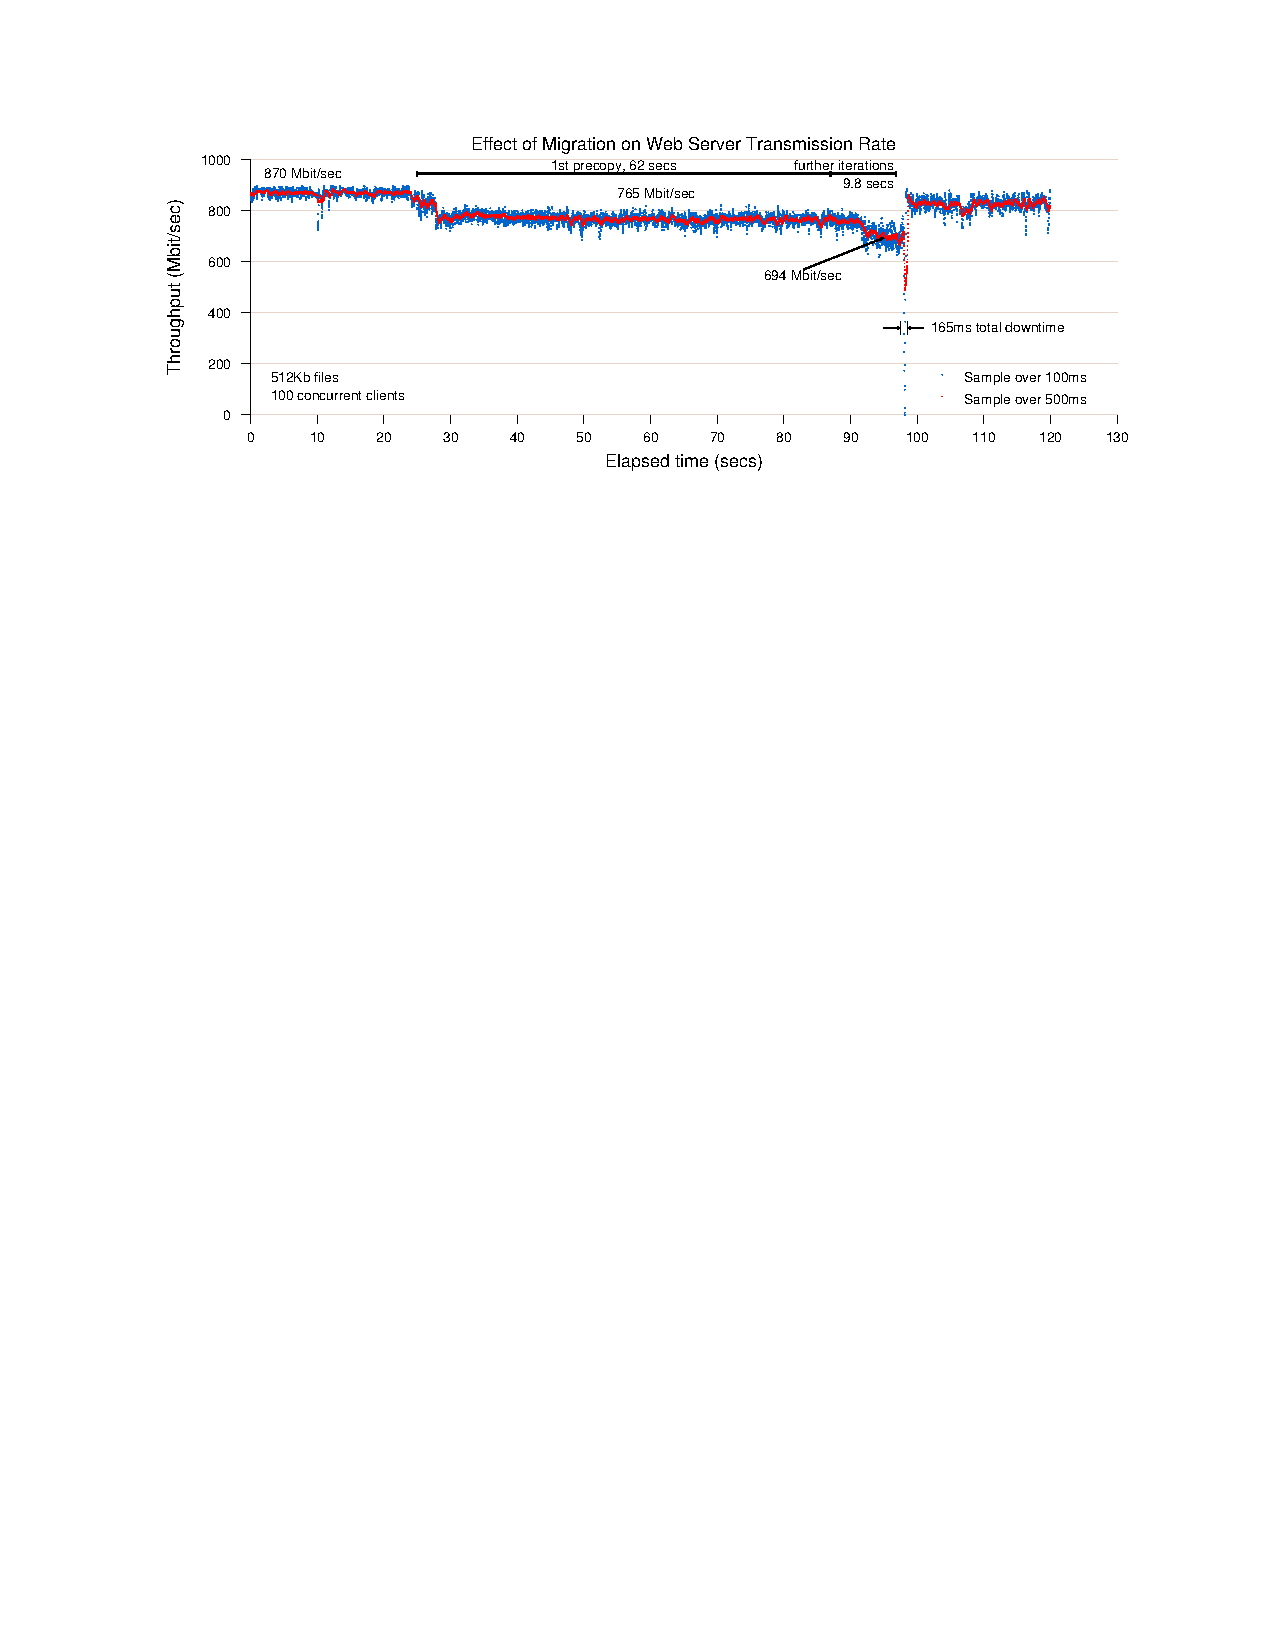
\includegraphics[width=15cm]{vmmigrate.pdf}
  \bicaption[WebServer虚拟机热迁移的网络开销]
    {WebServer虚拟机热迁移的网络开销\cite{livemigration}}
    {Network Overhead of WebServer VM Live Migration}
  \label{fig:livem}
\end{figure}

虚拟机的热迁移\cite{livemigration}分为本地资源的迁移和内存迁移。本地资源在源节点上,虽然像内存和处理器状态等数据可以通过网络发送到目的节点上,而本地的设备例如磁盘、网络接口则无法发送到目的节点,所以对这类资源需要特殊处理。在虚拟机热迁移的过程中,客户机的IP依然保存在TCP PCB(protocol control block,协议控制块)中,不会因为迁移而发生变化,只有其网卡的MAC地址(Media Access Control Address,媒体访问控制地址)发生了变化。源节点和目的节点经常处于同一个由单个交换机连接的局域网中,所以只要让目的节点在此局域网中广播一条包含IP地址的ARP(Address Resolution Protocol,地址解析协议,通过IP地址获知网卡的物理地址),当所有的机器接收到这条ARP消息后,即可得知客户机的新MAC地址,这样即可越过源节点,将所有的网络包发送给目的节点上的客户机。而对于本地的硬盘资源,依赖于设备整合(Device Consolidation)的解决方案,如NAS(Network-attached storage,网络存储),而NAS的地址不会因为虚拟机热迁移而发生变化,所以免去了磁盘迁移的需求。

虚拟机内存的迁移和容器的内存迁移类似,也有前拷贝、后拷贝两种选项,为了更短的下线时间,一般采用前拷贝。虚拟机内存迁移主要分为如下几个步骤:在开始虚拟机的热迁移之前,首先选择资源可以满足迁移来的客户机的且物理上更为临近的节点作为目标节点;接下来就是对内存页的循环拷贝,第一轮循环将客户机所有的物理页发送给目的节点,其余的循环重传上一个循环中被客户机修改的页。当第$i$个循环重传的页多于第$i-1$个循环时,将虚拟机冻结,传递CPU、设备等状态,再传递剩余的内存页,最后在目的节点上恢复虚拟机的执行。虚拟机开始执行后,不会产生远程缺页异常,且下线时间较短。对一个运行着WebServer的VM进行测试,只有165ms的下线时间,但是产生了巨大的网络开销,如图\ref{fig:livem}所示,在这个迁移过程中,从一开始的870Mbit/sec到最后的694Mbit/sec,如此大的网络开销持续了近100秒\cite{livemigration}。

综上所述,不同的迁移方式各有优劣,应用于不同的场景。容器热迁移具有较低的网络开销,但是下线时间较长;而虚拟机热迁移的下线时间极短,但由于其前拷贝的工作模式和虚拟机内存占用较高,具有极大的网络开销。数据中心在作出虚拟机迁移决定时一般较为慎重。

\section{本章小结}
本章介绍了进程的内存管理方式,以及NUMA架构及其内存自动平衡机制,为后文的理解奠定了知识基础;由于本课题基于巨型虚拟机,所以详述了巨型虚拟机的实现架构,特别是对性能影响较大的分布式共享内存的机制;分析了共享内存的性能瓶颈,并介绍了多内核架构操作系统对分布式共享内存良好的适应性,为高效地使用巨型虚拟机提供了指引;介绍了数据中心的概念和数据中心资源利用率的问题,并提出了三类解决该问题的方法,并详述了各个层面的迁移机制的优劣,进而影响到后文调度器的设计。